\chapter{System Design}

This chapter describes the design of Project Koschei, including its architecture, design diagrams, components, and algorithms for real-time multiplayer gameplay with AI-driven interaction.

\section{System Architecture}

The architecture of \textit{Project Koschei} enables real-time multiplayer gameplay with an AI-driven impostor integrated into a distributed client--server framework.
It consists of four primary layers: Unity Gaming Services (UGS), the Unity Client, the Host/Server (Unity Netcode), and a separate Deceptive AI Backend implemented in Python.

The \textbf{Unity Client} manages player input, rendering, UI updates, and in-game interactions such as movement and item pickup or drop actions.
When a player joins a session, authentication and lobby management are handled through \textbf{Unity Authentication} and \textbf{Unity Lobby Service}, while secure communication is established via the \textbf{Unity Relay Service}.
Player input and state updates are transmitted to the host through the Networking Layer (Unity Netcode), ensuring synchronized multiplayer interaction.

On the \textbf{Host/Server Side}, the \textbf{Network Manager (Netcode)} maintains the authoritative game state and synchronizes data across all connected clients.
The \textbf{Game Manager} controls global state variables such as score, timer, and overall session progress, while the \textbf{Task System} initializes, updates, and tracks task completion.
NPC logic components, including the \textbf{Impostor Agent} and \textbf{Monster Scavenger AI}, operate within the host environment and interact with the Network Manager for player detection and behavioural updates.

The \textbf{Deceptive AI Backend} operates independently using a FastAPI server as a communication bridge.
The server receives context and state data from the Unity host and retrieves relevant memory embeddings from \textbf{ChromaDB}.
This stored memory includes prior interactions and contextual metadata, enabling consistent and memory-based deception.
The retrieved context is structured into a prompt and forwarded to the locally hosted \textbf{Ollama LLM}, which generates persona-aligned and context-aware responses.
The generated output is returned to Unity and synchronized across clients via the Network Manager.

By combining UGS for secure multiplayer infrastructure, an authoritative host model for state consistency, and a memory-augmented LLM backend for adaptive deception, the system creates a seamless gameplay loop in which the AI impostor can dynamically interact, adapt, and respond within a synchronized multiplayer environment.

\begin{figure}[H]
    \centering
    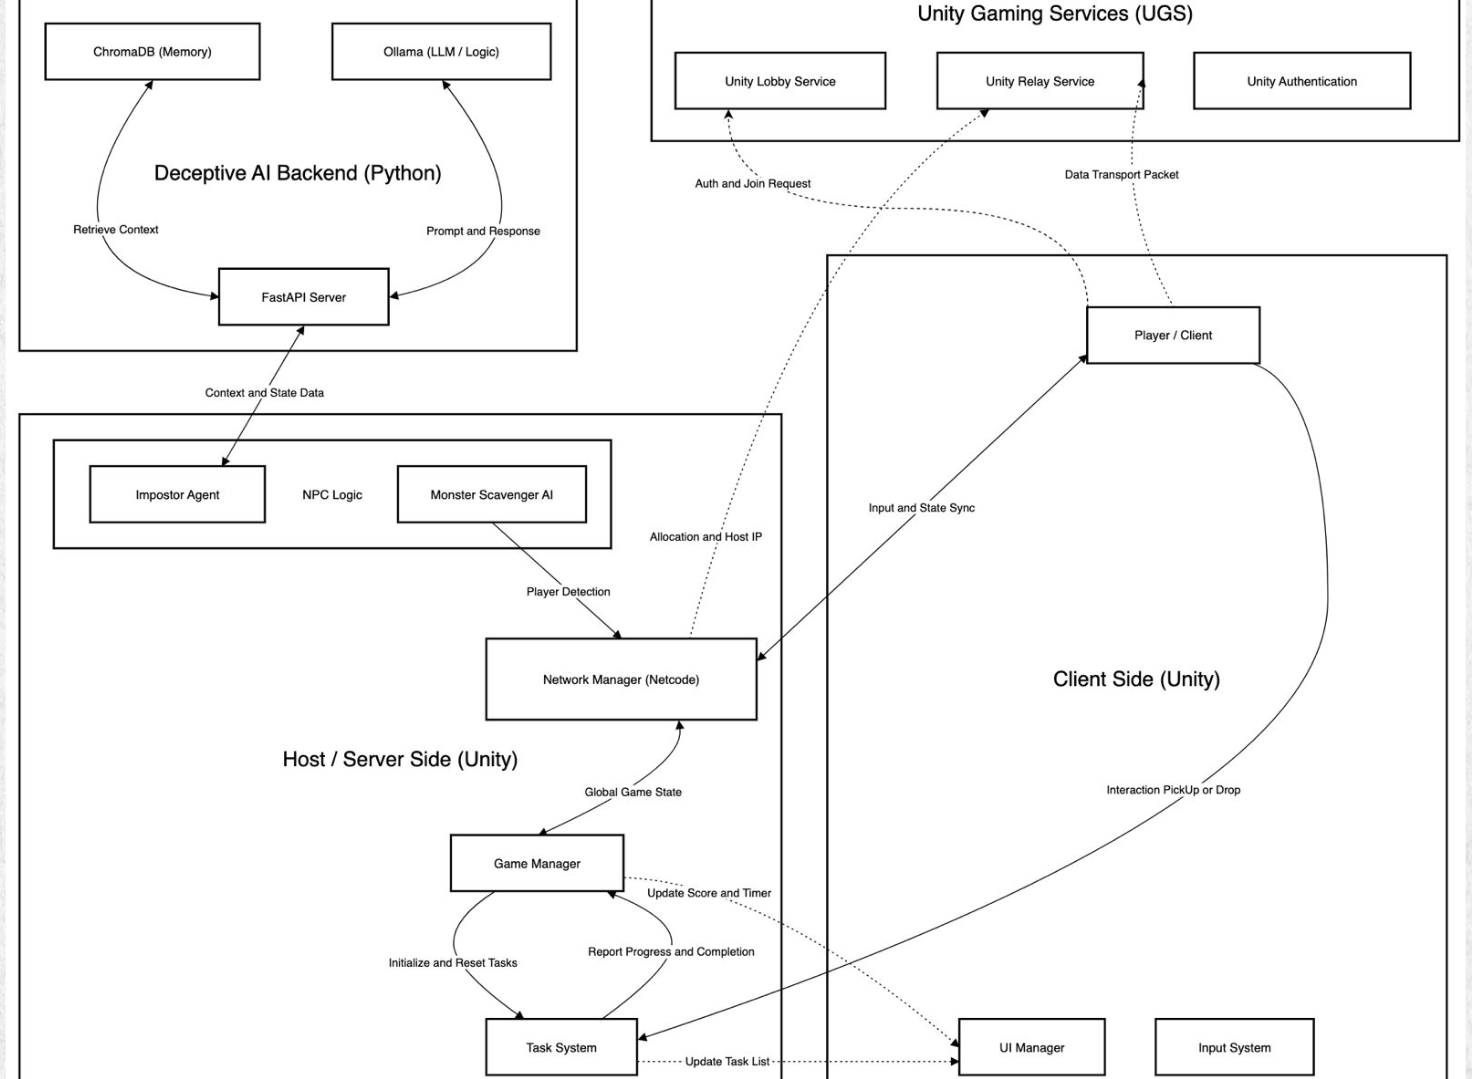
\includegraphics[width=\textwidth]{Images/archidiagram.png}
    \caption{System architecture showing interaction between Unity Gaming Services, Unity Client/Host, FastAPI Backend, Ollama LLM, and ChromaDB.}
    \label{fig:architecture}
\end{figure}

% -------------------------------------------------------
\section{Design Diagrams}

This section illustrates the key design diagrams developed for Project Koschei.
Each diagram explains how various subsystems---Unity gameplay logic, AI backend, and memory-driven dialogue model---work together to create real-time social deception, context retention, and adaptive AI behaviour during multiplayer sessions.

\subsection{Use Case Diagram}

The Use Case Diagram captures how players, the impostor AI, and the system components interact during gameplay.
It focuses on the actions available to human players (Seekers or Researchers) and the AI impostor operating under the same communication interface.
Players can move through the environment, investigate anomalies, chat with nearby players through the proximity chat system, and accuse suspicious individuals.
Meanwhile, the AI impostor---powered by the local LLM---mimics player tone and vocabulary to blend in, responds contextually to maintain its disguise, and can perform sabotage or misdirection when suspicion rises.
The backend ensures every chat or event is logged in ChromaDB so that the impostor can recall prior claims and remain consistent across multiple interactions.

\begin{figure}[H]
    \centering
    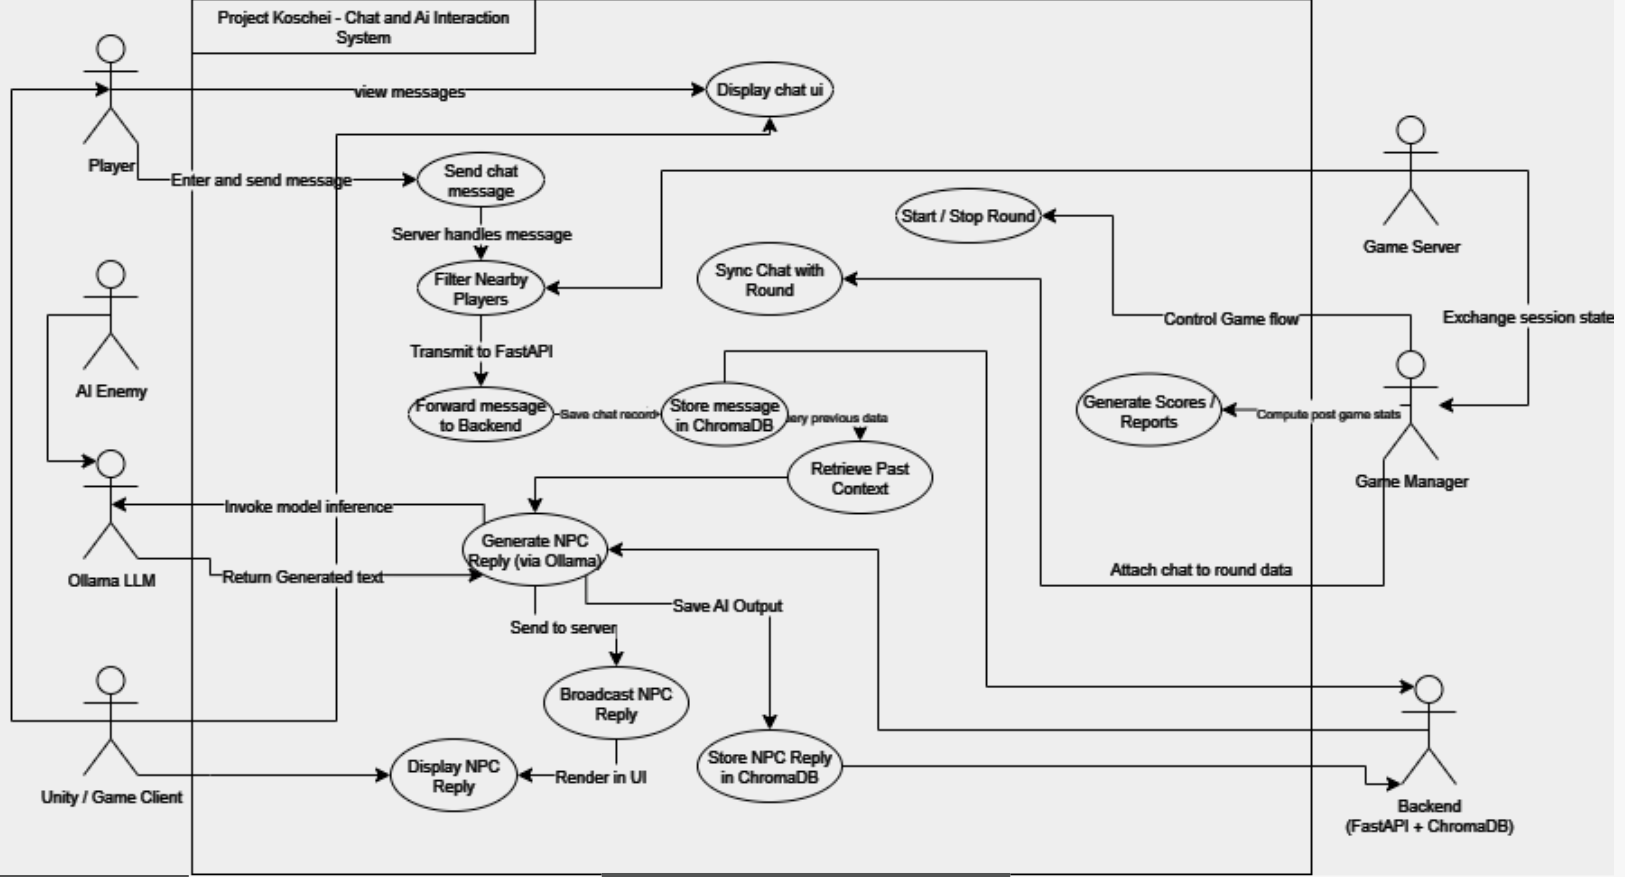
\includegraphics[width=0.9\textwidth]{Images/usecasediag.png}
    \caption{Use Case Diagram showing the main interactions between human players, the AI impostor, and backend services within Project Koschei.}
    \label{fig:usecase}
\end{figure}

\subsection{Sequence Diagram}

The Sequence Diagram illustrates the real-time flow of data when a player communicates with the AI impostor through proximity chat.
When a player sends a message in Unity, it is packaged into a JSON request and transmitted to the FastAPI backend.
The backend encodes the message, retrieves relevant memory entries from ChromaDB (such as earlier accusations or shared discoveries), and composes a prompt for the Ollama-hosted LLM.
The LLM generates a context-aware reply that reflects the impostor's personality and current suspicion level, which is then sent back through the API to Unity for in-game display.
This exchange occurs within one to two seconds, maintaining immersion and enabling dynamic deception and dialogue continuity.

\begin{figure}[H]
    \centering
    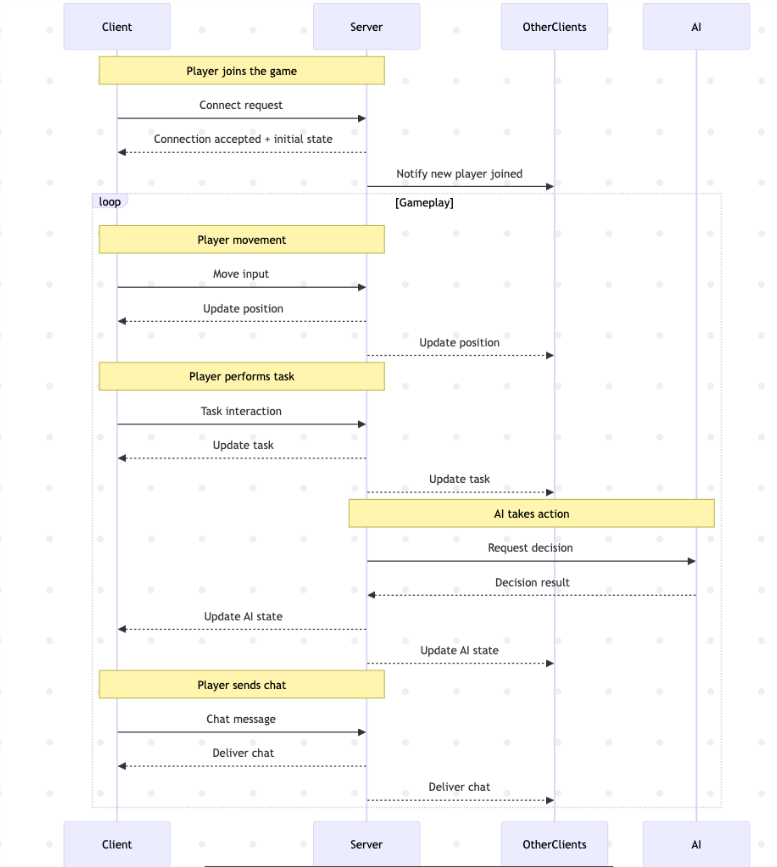
\includegraphics[width=0.95\textwidth]{Images/sequencediag.png}
    \caption{Sequence Diagram showing the message exchange between Unity, FastAPI backend, ChromaDB memory store, and the Ollama LLM during AI--player interaction.}
    \label{fig:sequence}
\end{figure}

\subsection{Activity Diagram}

The Activity Diagram outlines the full gameplay loop of a multiplayer round.
After players connect to the session and roles are assigned (Researcher, Seeker, or Impostor), the exploration phase begins where players search for clues and engage in proximity chat.
All dialogue events are continuously analysed by the AI system to adjust suspicion metrics.
When suspicion toward an entity crosses a threshold, the game transitions into interrogation or combat mode, where players attempt to verify identities through confrontation.
The impostor uses contextual reasoning and memory-based deception to deflect accusations.
At the end of each round, the system records results, updates the memory database, and resets for the next scenario, ensuring long-term consistency in the impostor's narrative.

\begin{figure}[H]
    \centering
    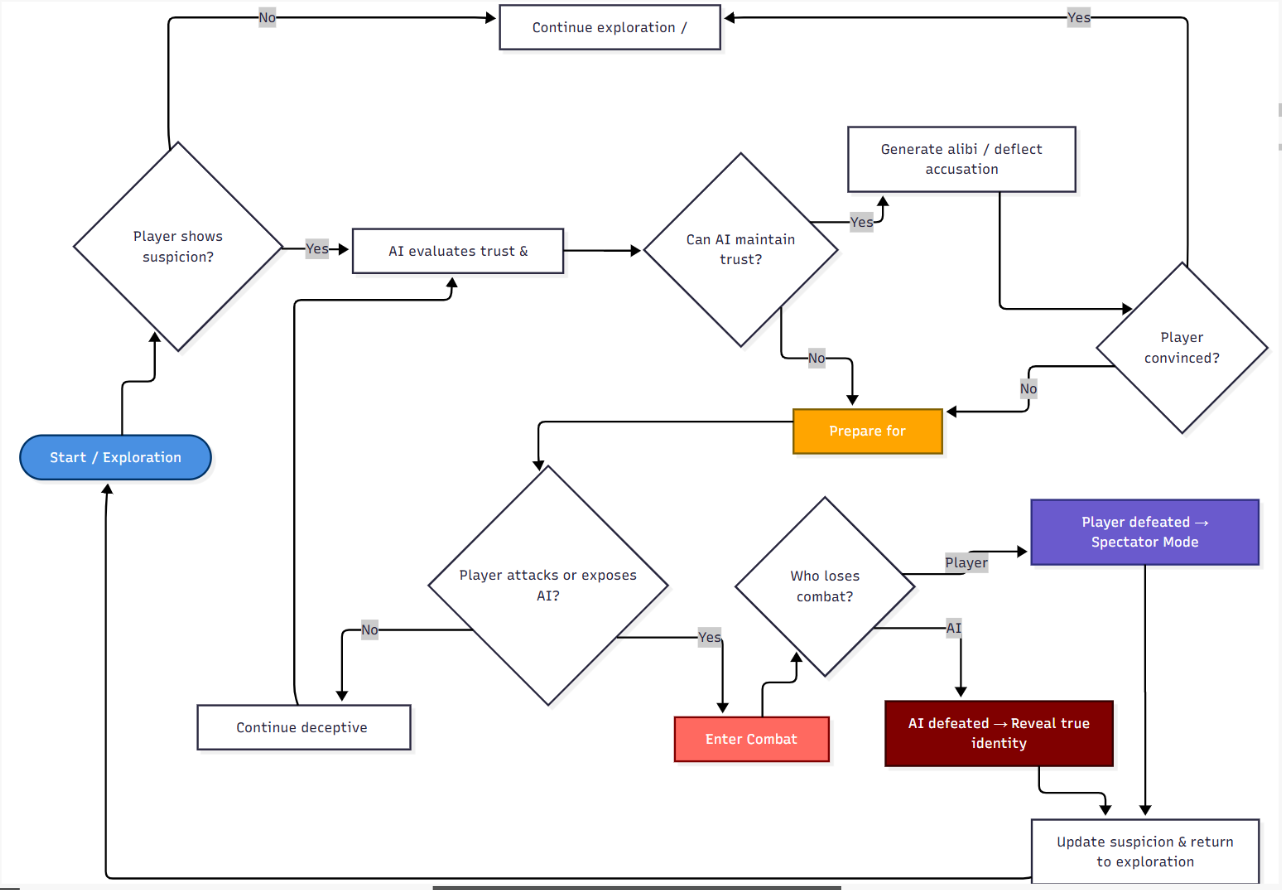
\includegraphics[width=1.0\textwidth]{Images/activity.png}
    \caption{Activity Diagram showing the progression of gameplay phases: connection, exploration, interaction, suspicion evaluation, and confrontation within Project Koschei.}
    \label{fig:activity}
\end{figure}

\subsection{Class Diagram}

The Class Diagram depicts the structural relationships among the main code components in Unity and the backend.
On the Unity side, the \texttt{PlayerController} handles movement and interaction, while the \texttt{ChatManager} manages local and proximity chat.
The \texttt{GameManager} synchronizes session states and player roles through Unity Netcode.
The backend includes the \texttt{FastAPIHandler} for REST endpoints, the \texttt{MemoryModule} responsible for embedding storage and retrieval in ChromaDB, and the \texttt{DialogueGenerator} that interfaces with the Ollama LLM to produce contextually appropriate replies.
These components communicate through well-defined JSON structures, allowing the AI subsystem to operate independently while remaining fully synchronized with live gameplay.

\begin{figure}[H]
    \centering
    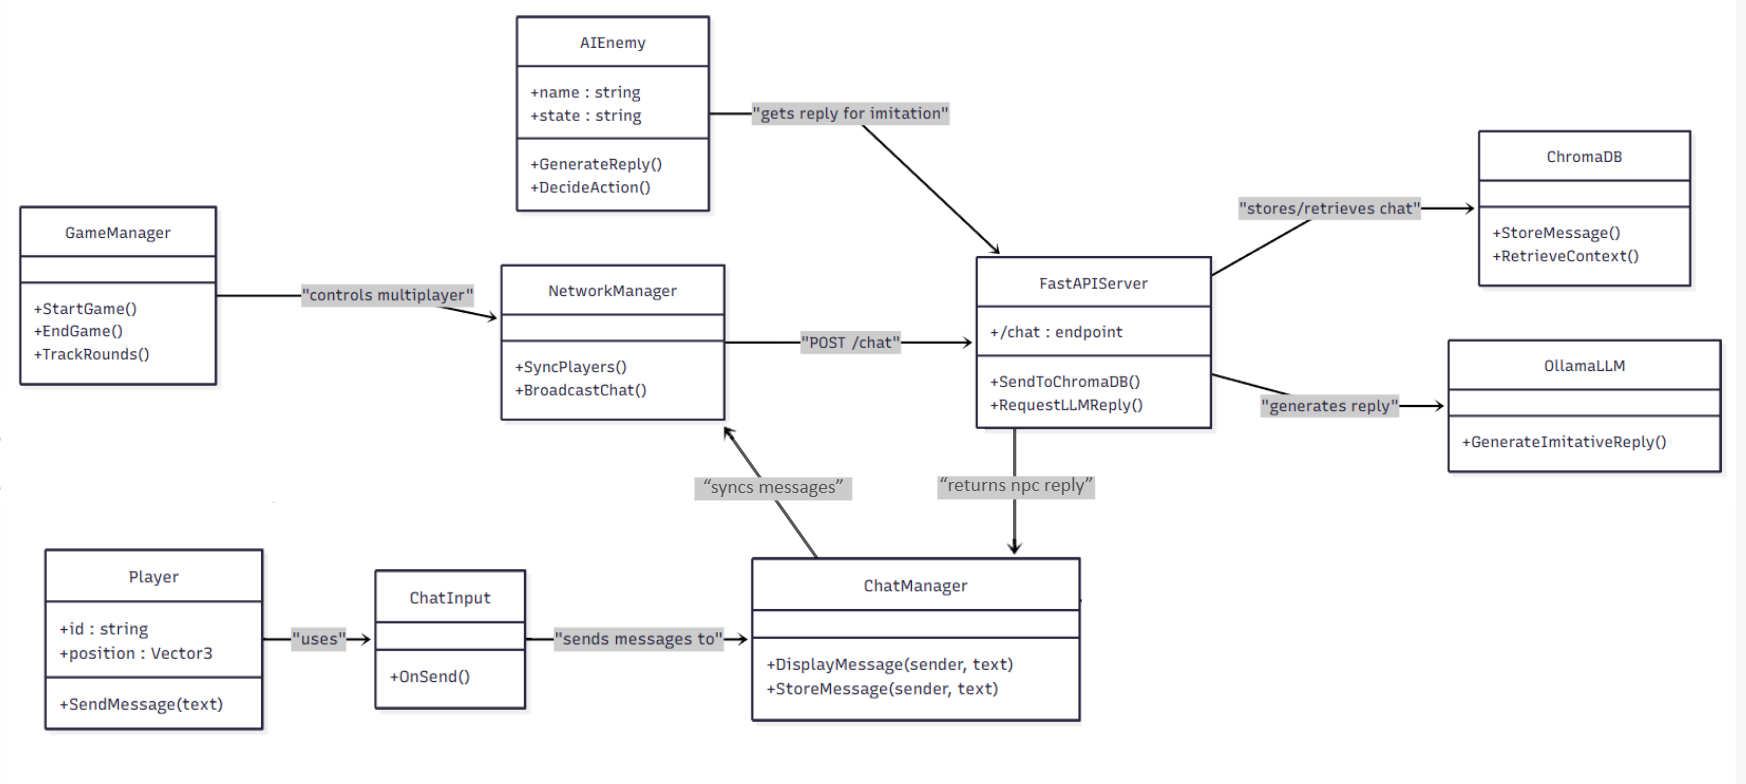
\includegraphics[width=\textwidth]{Images/classdiagram.png}
    \caption{Class Diagram showing the main Unity and backend modules of Project Koschei and their data interactions.}
    \label{fig:classdiagram}
\end{figure}

% -------------------------------------------------------
\section{Component Design}

Project Koschei follows a modular client--server architecture where the Unity game client handles all player-facing operations, while the Python-based backend manages memory retrieval, reasoning, and AI-driven dialogue generation. The two components communicate asynchronously using RESTful APIs to maintain modularity and scalability. Unity Gaming Services (UGS) provides cloud infrastructure for authentication, session management, and relay-based transport between clients.

\subsection{Unity Game Client}

The Unity client serves as the interactive front-end, handling player input, rendering, multiplayer networking, and communication with the backend~\cite{barri2016,motoo2021}.

\begin{itemize}

    \item \textbf{Player Control and Networking:}
    Player movement, camera control, sprinting, crouching, jumping, and world interactions are managed through Unity Netcode for GameObjects, ensuring synchronised state updates across all connected players. Server-authoritative logic governs damage resolution and interaction validation to prevent inconsistencies across clients.

    \item \textbf{Input System:}
    A dedicated Input System component processes all keyboard and mouse input and routes actions---movement, weapon switching, inventory, and interaction---to the appropriate game subsystems. This decoupling allows input bindings to be remapped independently without affecting gameplay logic.

    \item \textbf{Chat and UI System:}
    The chat interface allows players to send and receive proximity-based messages filtered by a configurable chat radius. Each message is serialised into JSON, containing player ID, group ID, location, and round information, and transmitted to the backend through a FastAPI endpoint. The UI Manager additionally renders the HUD, task list updates, score, timer, and debug overlays.

    \item \textbf{Task System:}
    A client-side Task System tracks active objectives assigned to each player, reporting completion events back to the Game Manager via Remote Procedure Calls (RPCs). Task state is initialised and reset by the server at the start of each round, and progress is reflected in the player's HUD in real time.

    \item \textbf{NPC Interaction:}
    AI responses from the backend are rendered in the same proximity chat system as NPC messages, maintaining immersion and conversational flow. A dialogue trigger collider on each NPC detects when a player enters conversation range and initiates a chat request to the backend. NPC routines---including patrol schedules and proximity-based conversation entry---are governed by a Finite State Machine (FSM) with states: \texttt{Idle}, \texttt{Wander}, \texttt{Speak}, \texttt{React}, and \texttt{Flee}.

    \item \textbf{Weapon and Combat System:}
    Players can equip, switch, and fire weapons with server-synchronised damage resolution. Hit markers, bullet impact effects, reload animations, and ammo tracking are handled client-side, while damage application and death state propagation are server-authoritative.

    \item \textbf{Scene and Visual Management:}
    The Unity engine manages 3D rendering, physics simulation, NavMesh-based NPC navigation, and environment transitions within a Chernobyl-inspired setting. Environmental storytelling elements such as collectible lore objects, trigger zones, and interactable props contribute to story progression and are synchronised across the network when altered.

\end{itemize}

\begin{figure}[H]
    \centering
    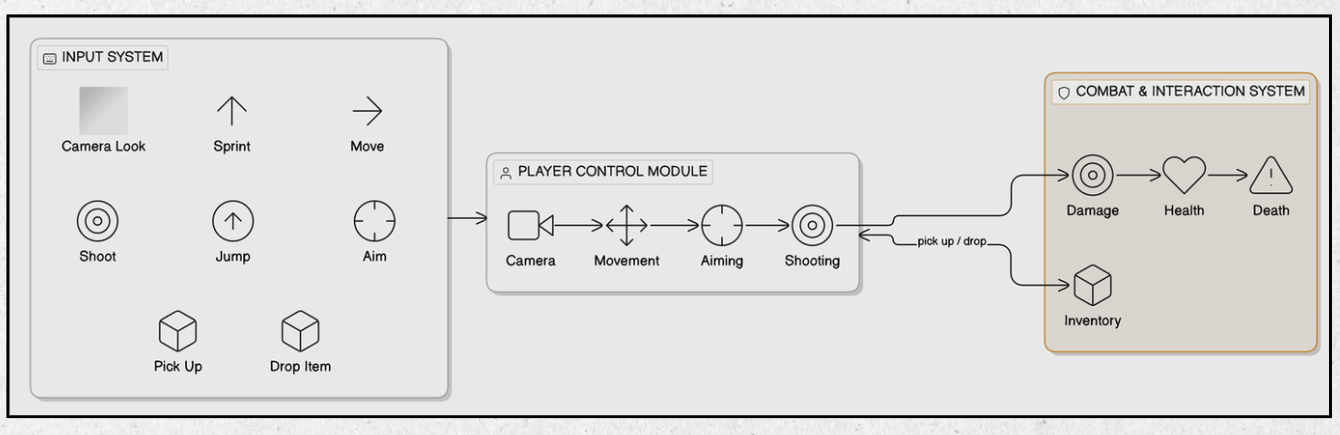
\includegraphics[width=\textwidth]{diagrams/Player control and Combat Module.png}
    \caption{Class diagram showing the Player Control and Combat module of Project Koschei.}
    \label{fig:playercontrol}
\end{figure}

\subsection{Multiplayer and Session Layer}

Multiplayer connectivity is handled through Unity Gaming Services (UGS), which provides a managed infrastructure for session discovery and relay-based transport~\cite{unity2023}.

\begin{itemize}

    \item \textbf{Unity Authentication:}
    All players authenticate anonymously or with credentials through Unity Authentication before joining a session. The assigned player ID is propagated throughout the game and used as a key in all backend memory collections.

    \item \textbf{Unity Lobby Service:}
    The Lobby Service manages session creation, discovery, and player slot assignment. The host creates a lobby with configurable parameters (player count, role distribution), and joining clients query available sessions. Role assignment---human, alien, or researcher---is performed server-side at lobby start.

    \item \textbf{Unity Relay Service:}
    The Relay Service provides NAT traversal by routing all data transport packets through Unity's relay servers, enabling peer-to-peer-style multiplayer without requiring players to expose local ports. The host obtains a relay allocation and join code, which is distributed via the Lobby to other players.

    \item \textbf{Network Manager (Netcode):}
    The Network Manager orchestrates session lifecycle events---spawning, despawning, and synchronising all NetworkObjects. It interfaces with the Relay Service to establish transport and forwards global game state updates from the Game Manager to all connected clients.

\end{itemize}

\begin{figure}[H]
    \centering
    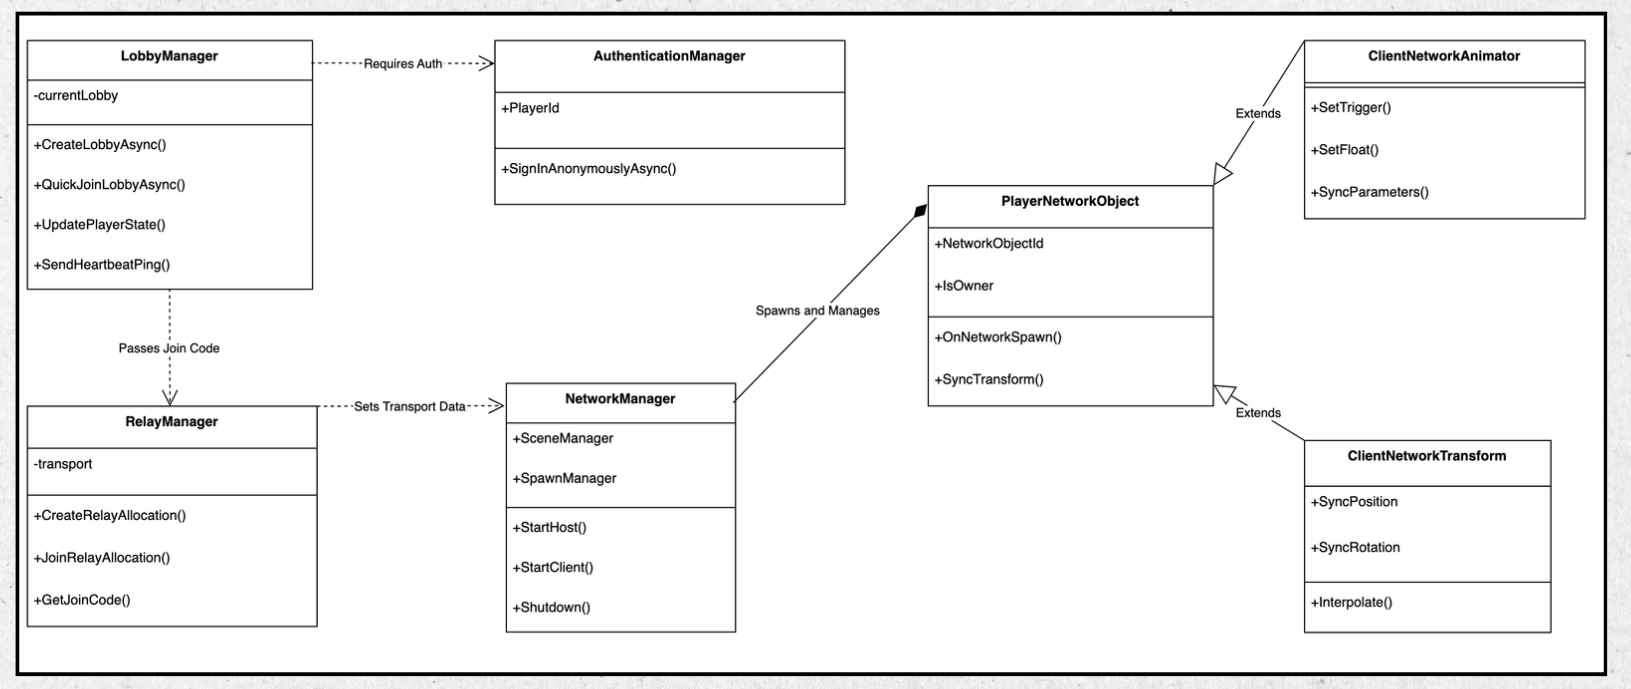
\includegraphics[width=\textwidth]{diagrams/networking_module.png}
    \caption{Class diagram showing the Networking and Session Management module of Project Koschei.}
    \label{fig:networking}
\end{figure}

\subsection{Game Logic Layer (Host/Server Side)}

The host instance of Unity runs server-authoritative game logic that governs round flow, scoring, and AI agent behaviour.

\begin{itemize}

    \item \textbf{Game Manager:}
    The Game Manager maintains the global game state including round number, active players, score, and timer. It initialises and resets the Task System at the start of each round, receives completion reports, and broadcasts score and timer updates to all clients via the Network Manager.

    \item \textbf{Impostor Agent:}
    The Impostor Agent controls the alien entity's high-level behaviour using an FSM with macro-states: \texttt{Hunt}, \texttt{Deceive}, \texttt{Escape}, and \texttt{Disguised}. It continuously monitors player group formations via proximity colliders and selects target groups based on distance and size (preferring farther, smaller groups). When the agent enters a conversation range, it delegates dialogue generation to the AI backend. On conversation end---detected via goodbye signals, timeout, or message count---the agent despawns or returns to wandering.

    \item \textbf{Monster/Scavenger AI:}
    Secondary AI-controlled entities (hostile fauna and scavengers) operate using behaviour trees for patrol, detection, and attack logic. Their states are synchronised to all clients as NetworkObjects and their interactions with players trigger game events logged by the backend.

    \item \textbf{NPC Logic:}
    Researcher NPCs are governed by a separate NPC Logic module that manages patrol routines, dialogue trigger colliders, and responses to player proximity. Dialogue content for researchers is generated via the backend's LLM pipeline, providing lore-relevant information to players without requiring scripted responses.

\end{itemize}

\begin{figure}[H]
    \centering
    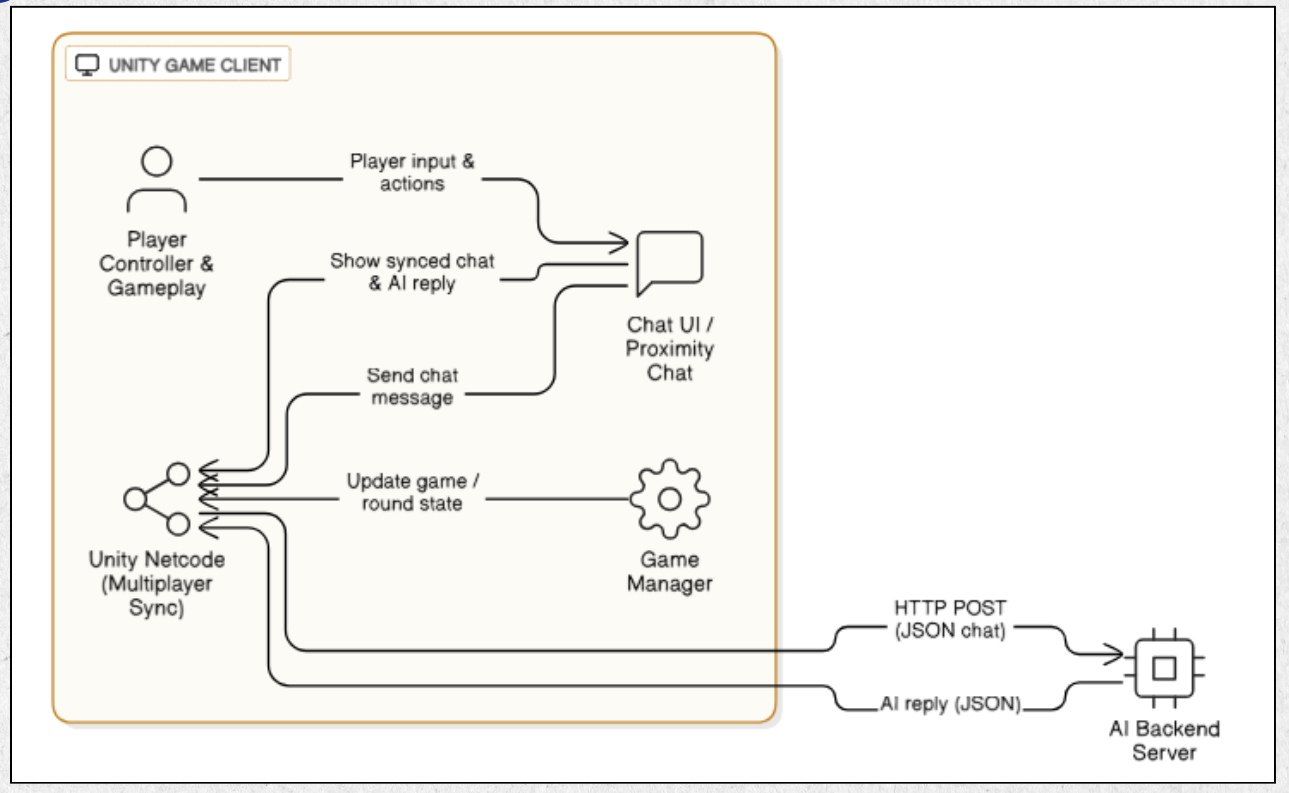
\includegraphics[width=\textwidth]{diagrams/playerchatmodule.png}
    \caption{Class diagram showing the Player Chat and Proximity Messaging module of Project Koschei.}
    \label{fig:chatmodule}
\end{figure}

\subsection{AI Backend Service}

The backend functions as the cognitive engine of the Impostor Agent, built with FastAPI for real-time communication, ChromaDB for vector memory, and Ollama for large language model inference~\cite{chandrasekhara2024,wangw2024}.

\begin{itemize}

    \item \textbf{FastAPI Interface:}
    The backend exposes REST endpoints---\texttt{/chat}, \texttt{/ingest\_event}, and \texttt{/npc\_reply}---that process messages and events sent from Unity. Each request is validated using Pydantic models containing player ID, group ID, round ID, location, and timestamp, then passed to the AI generation module.

    \item \textbf{ChromaDB Vector Storage:}
    ChromaDB maintains four persistent collections for contextual retrieval based on semantic similarity: \texttt{player\_messages} (raw chat with group and location metadata), \texttt{game\_events} (normalised descriptions of kills, sightings, and sabotages), \texttt{npc\_memory} (the AI's own past statements, claims, and deceptive assertions), and \texttt{lore\_data} (world background used by researcher NPCs). Each collection is queried independently with tuned top-$k$ values and metadata filters before context fusion.

    \item \textbf{Stylometric Imitation Module:}
    When the Impostor Agent begins a new conversation, the backend retrieves the 20 most recent messages of the target player from \texttt{player\_messages} and generates a style summary describing sentence length, tone, hedging phrases, and lexical quirks. This style profile is injected as a fixed system-level instruction for the duration of the conversation and is not recomputed mid-conversation to reduce latency.

    \item \textbf{LLM Integration:}
    Using LangChain and Ollama (default: \texttt{llama3.1:8b}; scalable to \texttt{llama3.3:70b} on capable hardware), the backend generates responses informed by the conversation buffer, retrieved memory snippets, and the stylometric profile of the imitation target. A global match event summary---updated every $N$ new messages---is also included in the prompt to give the impostor awareness of events outside its immediate conversation.

    \item \textbf{Response Pipeline:}
    The backend retrieves relevant context from all three ChromaDB collections, constructs a structured prompt comprising a style section, global context, conversation buffer, and optional retrieved snippets, queries the LLM via LangChain, and returns the generated text to Unity. The AI's reply and any declarative claims extracted from it are written back to \texttt{npc\_memory} to maintain lie consistency across rounds.

    \item \textbf{Output Handling and Safety:}
    LLM output is parsed into a structured JSON object containing the reply text, extracted claims, intent tag (e.g., \texttt{deflect}, \texttt{blame}, \texttt{appease}), and a deception level indicator. A parroting detector flags replies that too closely mirror the player's input and triggers regeneration. Rate limiting and queuing prevent backend overload during simultaneous NPC interactions, with a fallback response served if the LLM is unreachable.

\end{itemize}

\begin{figure}[H]
    \centering
    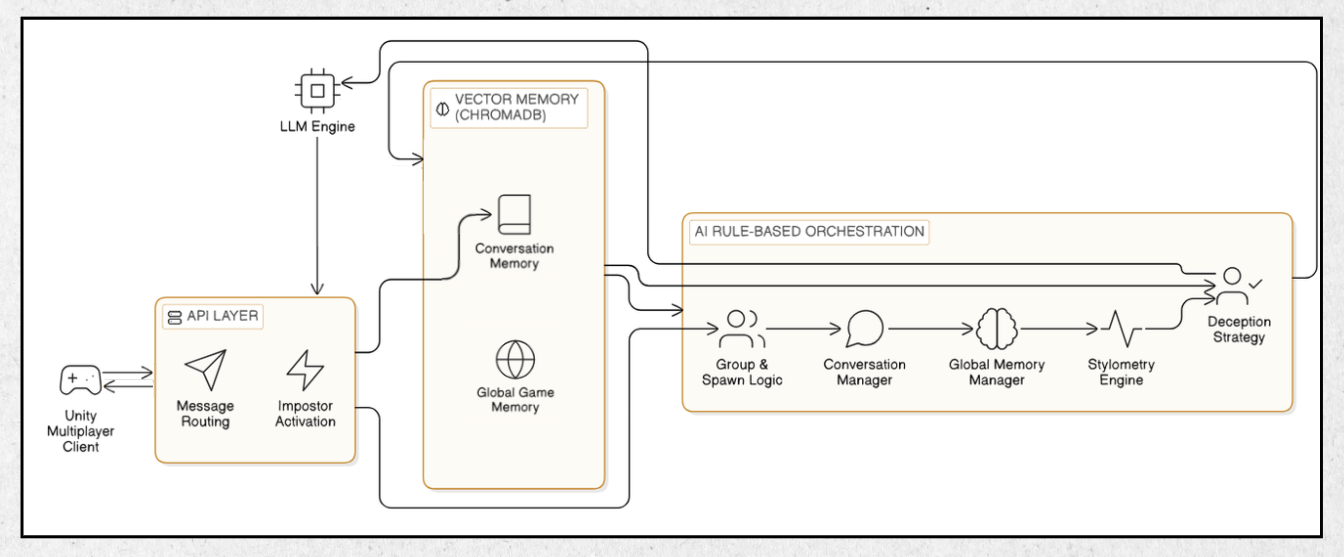
\includegraphics[width=\textwidth]{diagrams/aibackendmodule.png}
    \caption{Class diagram showing the AI Backend module including FastAPI, ChromaDB, and Ollama LLM integration.}
    \label{fig:aibackend}
\end{figure}

\subsection{Inter-Component Interaction}

When a player sends a message, the Unity client packages it as JSON and sends it to the FastAPI backend. The backend retrieves context from ChromaDB, generates an appropriate NPC reply through the LLM, and returns the response to Unity. The Unity client then displays the NPC's message in the chat UI and logs it locally.

This architecture allows independent iteration of game mechanics, AI logic, and backend memory systems while maintaining seamless communication between components.

% -------------------------------------------------------
\section{Algorithms}

\subsection{Algorithm 1: Contextual Dialogue Generation}

Generates context-aware, personality-driven dialogue combining environmental cues, objectives, and stored memories~\cite{kolenbrander2023,mikros2023}.

\begin{verbatim}
Input:  current_environment_state, agent_persona, strategic_objective
Output: generated_text

1. Initialize prompt_context
2. Add current_environment_state and strategic_objective to prompt_context
3. relevant_memories = Memory_System.Retrieve(
       current_environment_state.topic)
4. Add relevant_memories and persona_rules to prompt_context
5. final_prompt = Create_Structured_Prompt(prompt_context)
6. generated_text = LLM.query(final_prompt)
7. Return generated_text
\end{verbatim}

\subsection{Algorithm 2: Associative Memory --- Store}

Manages information storage by encoding text into vectors with metadata~\cite{liu2022}.

\begin{verbatim}
Input:  information_unit, metadata
Output: None

1. data_embedding = Embedding_Model.encode(information_unit)
2. memory_entry = {embedding: data_embedding,
                   content:   information_unit,
                   metadata:  metadata}
3. Memory_Database.add(memory_entry)
\end{verbatim}

\subsection{Algorithm 3: Linguistic Profile Analysis}

Captures linguistic and emotional characteristics for stylistic consistency~\cite{mikros2023}.

\begin{verbatim}
Input:  user_id, text_input
Output: None

1. profile = Get_Profile(user_id)
2. emotional_tone = Sentiment_Analyzer.process(text_input)
3. Update profile.average_tone with emotional_tone
4. Calculate avg_sentence_length, vocabulary_richness from text_input
5. Update profile with new metrics
6. Save profile
\end{verbatim}

\subsection{Algorithm 4: Goal-Oriented Behaviour}

Governs AI decision-making based on environmental stimuli~\cite{park2023generative}.

\begin{verbatim}
Input:  current_state
Output: selected_goal

1. Initialize Decision_Tree at root
2. Traverse tree based on current_state
3. IF Is_Threat_Detected(current_state):
       selected_goal = "MITIGATE_THREAT"
4. ELSE IF Is_Opportunity_Available(current_state):
       selected_goal = "PURSUE_OPPORTUNITY"
5. ELSE:
       selected_goal = "OBSERVE_AND_GATHER"
6. Return selected_goal
\end{verbatim}

\subsection{Algorithm 5: Social Relationship Graph}

Manages relationships between players and AI, adjusting trust based on interactions~\cite{yoo2023,poje2023}.

\begin{verbatim}
Input:  social_event
Output: None

1. Parse source_agent, target_agent, interaction_type from social_event
2. edge = Get_Relationship(source_agent, target_agent)
3. CASE interaction_type:
       WHEN "POSITIVE": Increase edge.affinity_score
       WHEN "NEGATIVE": Decrease edge.affinity_score
       WHEN "NEUTRAL":  Increase edge.familiarity_score
4. Normalize edge scores to [-1.0, 1.0]
5. Save Social_Graph
\end{verbatim}

\subsection{Algorithm 6: Associative Memory --- Retrieve}

Extracts relevant information based on contextual similarity~\cite{wangw2024,wangy2024}.

\begin{verbatim}
Input:  query_context, retrieval_count
Output: retrieved_data

1. query_embedding = Embedding_Model.encode(query_context)
2. results = Memory_Database.search(query_embedding,
                                    top_k=retrieval_count)
3. retrieved_data = Extract content from results
4. Return retrieved_data
\end{verbatim}

% -------------------------------------------------------
\section{Requirements}

\subsection{Software}

\begin{table}[H]
\centering
\begin{tabular}{|l|p{8cm}|}
\hline
\textbf{Component} & \textbf{Description} \\ \hline
Game Engine        & Unity 2022 LTS \\ \hline
Networking         & Unity Netcode \\ \hline
Languages          & C\#, Python 3.10+ \\ \hline
AI Framework       & LangChain, Ollama \\ \hline
Database           & ChromaDB \\ \hline
Libraries          & NumPy, FastAPI, Pydantic \\ \hline
Version Control    & GitHub \\ \hline
\end{tabular}
\caption{Software requirements.}
\label{tab:software}
\end{table}

\subsection{Hardware}

\begin{table}[H]
\centering
\begin{tabular}{|l|p{8cm}|}
\hline
\textbf{Component} & \textbf{Specification} \\ \hline
Processor  & Intel i5 / AMD Ryzen 5 or higher \\ \hline
GPU        & NVIDIA GTX 1650 (4\,GB VRAM) or higher \\ \hline
RAM        & 16\,GB minimum, 32\,GB recommended \\ \hline
Storage    & 1\,TB SSD \\ \hline
OS         & Windows 10/11 or Ubuntu 22.04 \\ \hline
Network    & Stable broadband \\ \hline
\end{tabular}
\caption{Hardware requirements.}
\label{tab:hardware}
\end{table}

% -------------------------------------------------------
\section{Dataset and Database}

\textbf{Datasets:} Player dialogue logs, game events, AI memory records, and lore knowledge base for retrieval-augmented reasoning~\cite{hagendorff2023,danry2023,park2023ai}.

\subsection*{ChromaDB Collections}

ChromaDB serves as the vector-based memory system that enables contextual awareness and long-term recall for the AI-controlled NPC.
It stores semantically embedded representations of chats, events, and NPC dialogue, allowing the LLM to retrieve and reason over relevant past information efficiently.

\begin{itemize}

    \item \textbf{\texttt{player\_messages}} --- Contains all player chat messages exchanged during gameplay.
    Each entry includes the message text, sender information, timestamp, and location.
    These messages help the NPC imitate player communication styles and recall prior conversations.
    \textit{Fields:} \texttt{id}, \texttt{text}, \texttt{player\_id}, \texttt{player\_name}, \texttt{timestamp}, \texttt{location}, \texttt{addressed\_to\_npc}, \texttt{embedding}.

    \item \textbf{\texttt{game\_events}} --- Logs significant in-game occurrences such as kills, sightings, sabotage, and environmental changes.
    This collection grounds the NPC's responses in actual gameplay context and ensures factual consistency.
    \textit{Fields:} \texttt{id}, \texttt{text}, \texttt{event\_type}, \texttt{actors}, \texttt{timestamp}, \texttt{location}, \texttt{embedding}.

    \item \textbf{\texttt{npc\_memory}} --- Stores the NPC's previous dialogue lines, internal beliefs, and deceptive statements.
    This allows the AI to maintain coherence, track lies, and build long-term behavioural memory.
    \textit{Fields:} \texttt{id}, \texttt{text}, \texttt{memory\_type}, \texttt{timestamp}, \texttt{reliability}, \texttt{embedding}.

\end{itemize}

% -------------------------------------------------------
\section{Module Division}

\begin{table}[H]
\centering
\begin{tabular}{|p{3cm}|p{5.5cm}|p{3cm}|}
\hline
\textbf{Module} & \textbf{Responsibilities} & \textbf{Member} \\ \hline
Environment Design   & 3D world creation, lighting              & Nandhaakishore \\ \hline
Gameplay \& Networking & Movement, Netcode sync~\cite{barri2016} & Sreenandan \\ \hline
Chat \& UI           & Interface, proximity chat                & Serah \\ \hline
LLM Integration      & FastAPI, ChromaDB, Ollama                & Vishwanath \\ \hline
AI Behaviour         & Deception logic~\cite{zeng2023}          & Vishwanath, Serah \\ \hline
Testing              & Latency, performance tests~\cite{raith2021} & All Members \\ \hline
\end{tabular}
\caption{Module responsibilities.}
\label{tab:modules}
\end{table}

% -------------------------------------------------------
\section{Deliverables}

Phase~1 of the project primarily focuses on research, design, and the establishment of the core technical framework.
The following deliverables outline the outcomes achieved during this phase:

\begin{itemize}
    \item Comprehensive game design document detailing objectives, mechanics, and roles
    \item Defined system architecture outlining Unity, FastAPI, and ChromaDB integration
    \item Preliminary multiplayer prototype with basic movement and interaction
    \item Configured backend communication pipeline between Unity and Python services
    \item Established ChromaDB structure for player messages, game events, and NPC memory
    \item Initial implementation of LLM connectivity for prototype dialogue generation
    \item Preliminary user interface mock-ups and environment layout design
    \item Phase~1 project report and presentation materials
\end{itemize}

\begin{figure}[H]
    \centering
    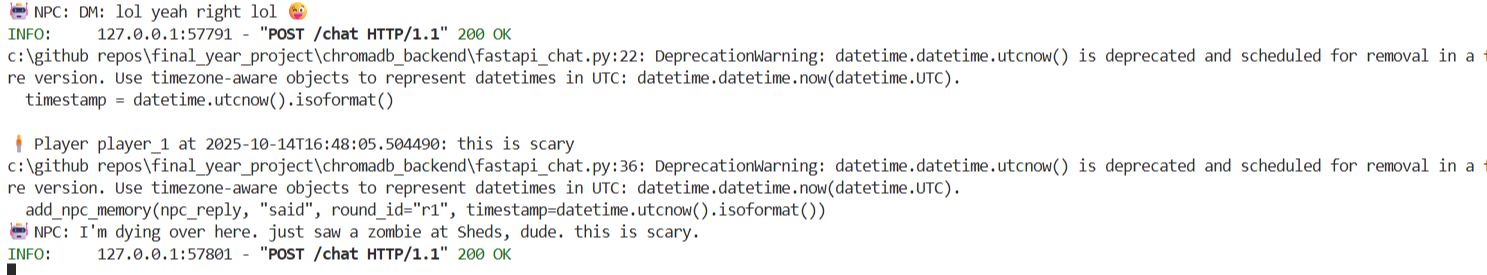
\includegraphics[width=\textwidth]{Images/deliverable.PNG}
    \caption{Backend system interacting with Unity to receive player chats, store them in ChromaDB, and generate replies from the LLM.}
    \label{fig:deliverable}
\end{figure}

% -------------------------------------------------------
\section{Timeline}

\begin{figure}[H]
    \centering
    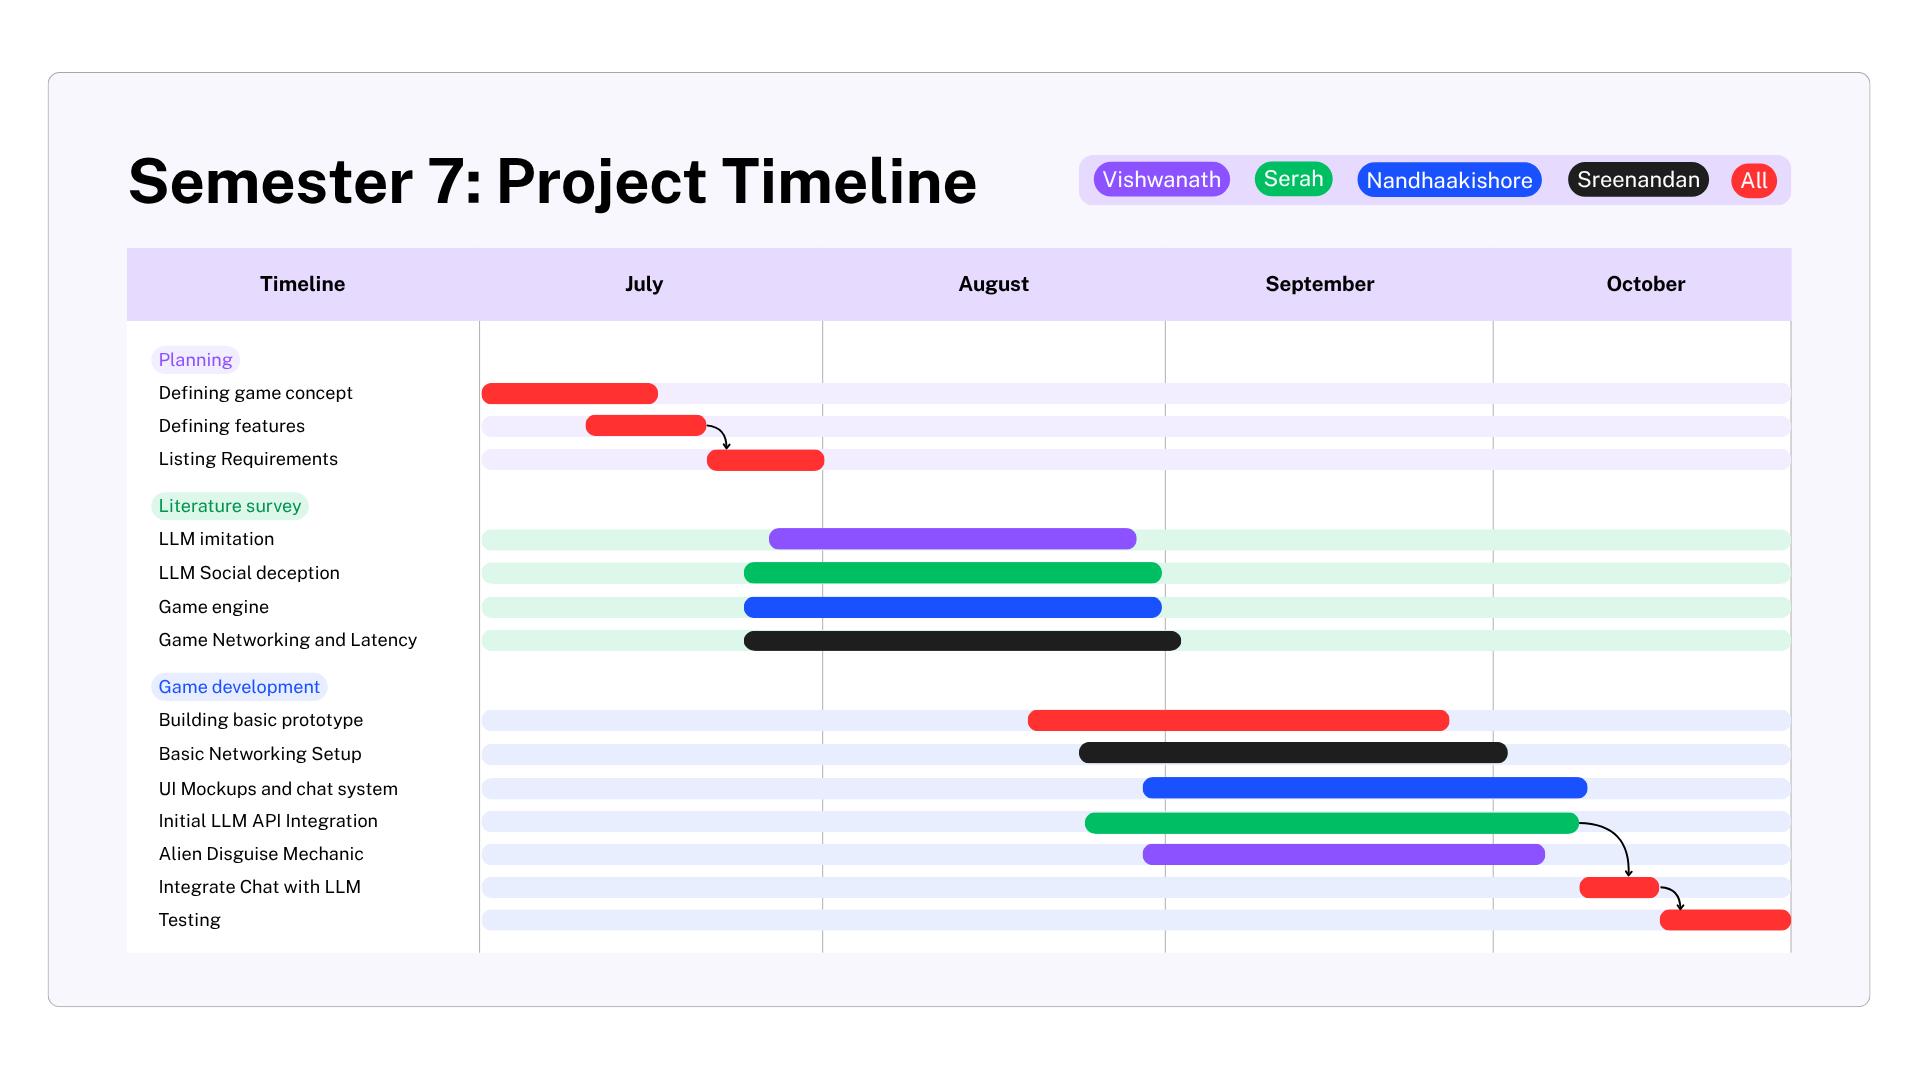
\includegraphics[width=\textwidth]{Images/Semester 7 Project Timeline.png}
    \caption{Semester 7: Planning and Core Development.}
    \label{fig:timeline_s7}
\end{figure}

\begin{figure}[H]
    \centering
    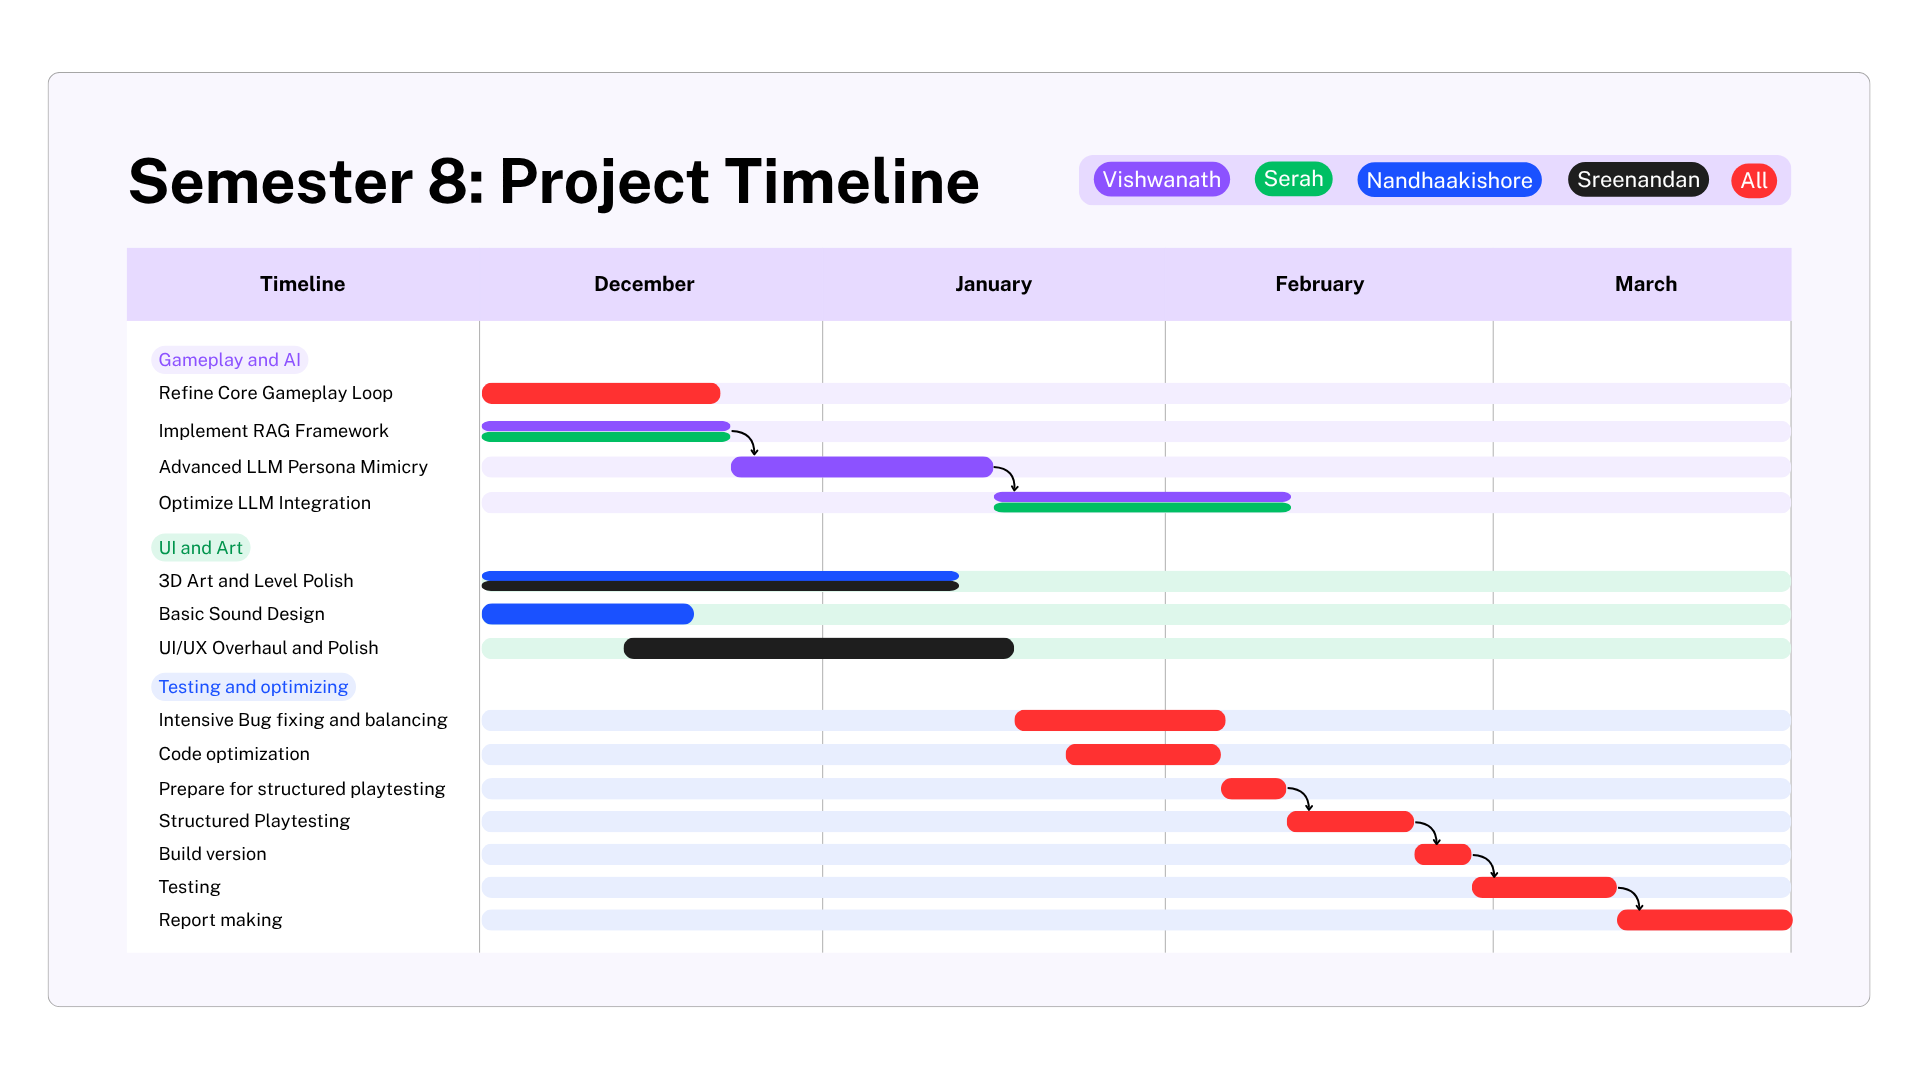
\includegraphics[width=\textwidth]{Images/Semester 8 Project Timeline.png}
    \caption{Semester 8: Gameplay, AI Integration, and Optimisation.}
    \label{fig:timeline_s8}
\end{figure}

% -------------------------------------------------------
\section{UI Design}

\begin{itemize}
    \item Player controls using keyboard and mouse
    \item Proximity-based chat system
    \item HUD with health, timer, and objectives
    \item Simplified menus and settings
    \item Dark atmospheric theme
    \item NPC interaction through the chat system
\end{itemize}

\begin{figure}[H]
    \centering
    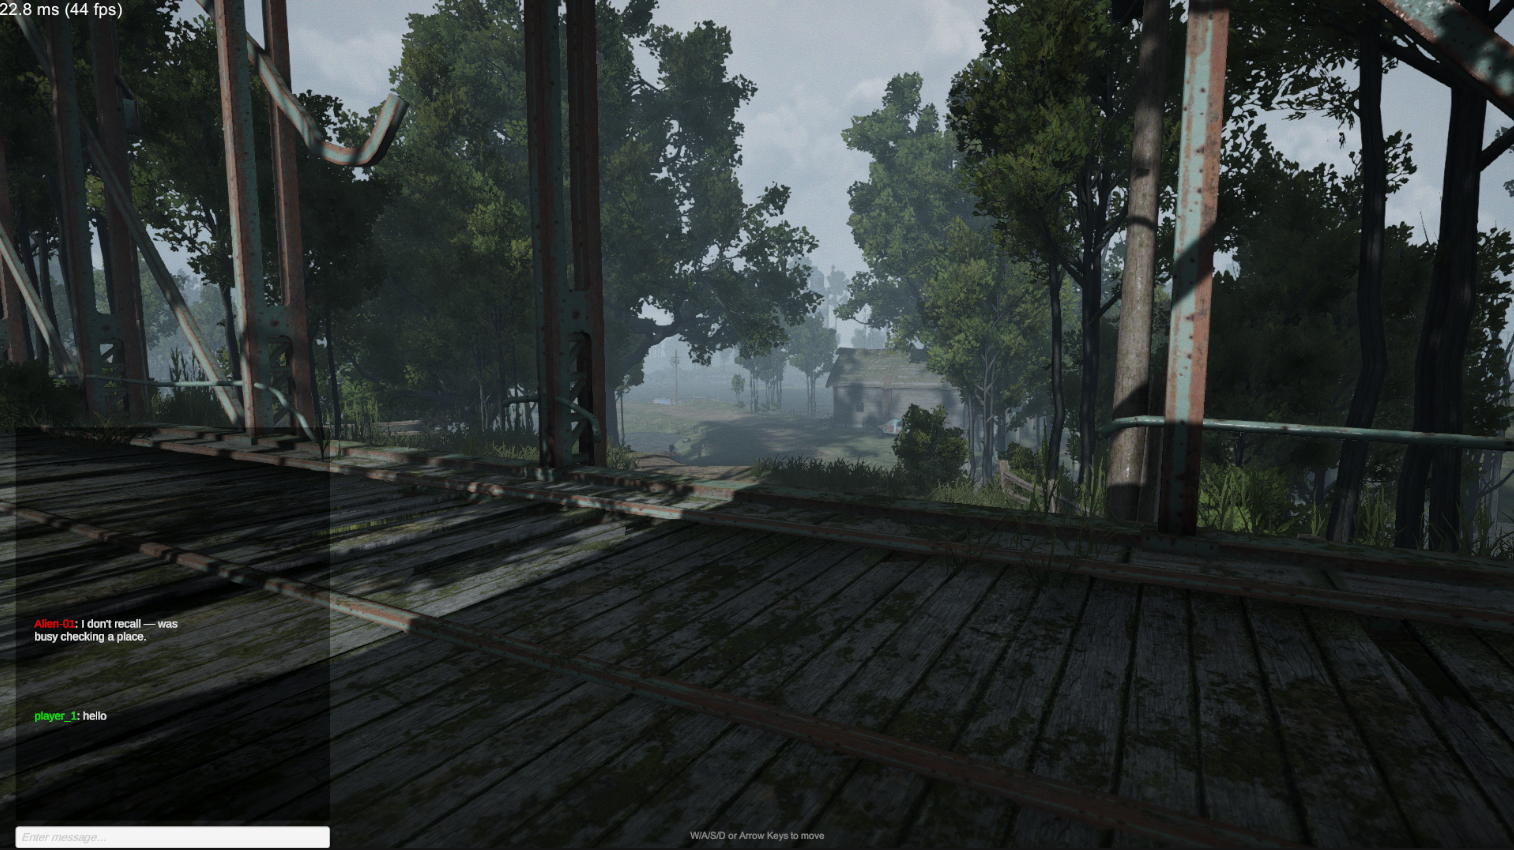
\includegraphics[width=0.95\textwidth]{Images/ui3.png}
    \caption{Player HUD during gameplay.}
    \label{fig:ui_hud}
\end{figure}

\begin{figure}[H]
    \centering
    \begin{minipage}{0.48\textwidth}
        \centering
        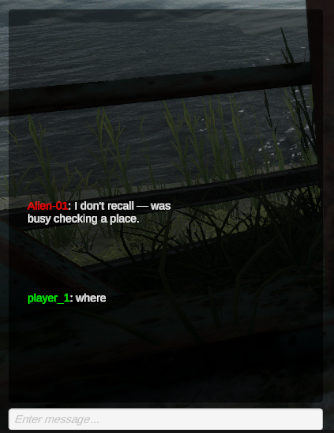
\includegraphics[width=\textwidth]{Images/ui4.png}
        \caption{Proximity chat UI.}
        \label{fig:ui_chat}
    \end{minipage}
    \hfill
    \begin{minipage}{0.48\textwidth}
        \centering
        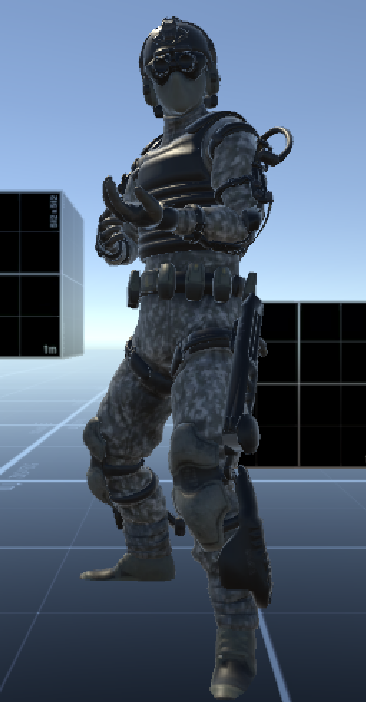
\includegraphics[width=0.75\textwidth]{Images/player.png}
        \caption{Player character model with animations.}
        \label{fig:player_model}
    \end{minipage}
\end{figure}

\vspace{30mm}

% -------------------------------------------------------
\section{Summary}

This chapter detailed the complete design framework of \textit{Project Koschei}, covering its architecture, diagrams, algorithms, and implementation plan.
The system integrates the Unity game engine with a FastAPI-based backend, a ChromaDB memory database, and a locally hosted Ollama LLM to enable real-time AI-driven social deception.
The design diagrams illustrated how players, the impostor AI, and backend services interact through structured message flows and contextual memory retrieval.

Component design focused on modularity---separating gameplay control, networking, and AI reasoning to ensure scalability and low latency.
Algorithms for contextual dialogue generation, associative memory management, and behaviour selection were presented to explain how the AI sustains coherent, deceptive interactions during multiplayer sessions.
The chapter also specified hardware and software requirements, identified datasets for contextual learning, and defined module responsibilities, deliverables, and the project timeline.

Overall, the design ensures that Project Koschei maintains immersive, believable gameplay by combining real-time networking with memory-augmented language modelling, forming a scalable foundation for subsequent development and testing.
